\section{Design}\label{sec:method}

\begin{figure*}[t]
\centering
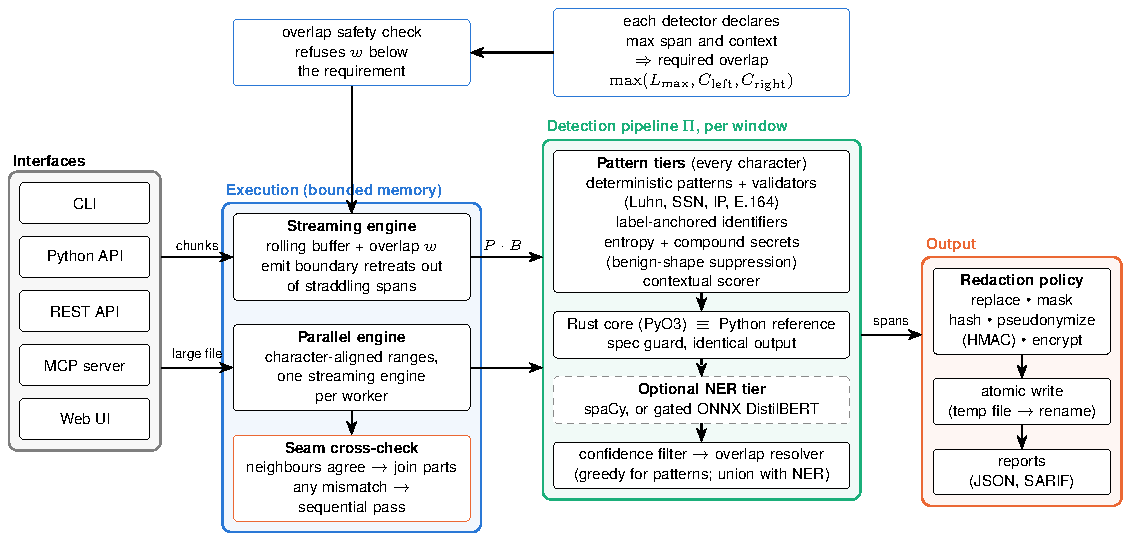
\includegraphics[width=\textwidth]{fig_architecture.pdf}
\caption{System architecture. Interfaces feed text to the streaming engine or, for a large file, to the parallel engine, whose workers each run a streaming engine and whose seams are cross-checked. Each window passes through the detection pipeline $\Pi$: the pattern tiers run on every character, on the Rust core or the identical Python reference. The dashed named-entity tier (spaCy) is optional. The resolver produces disjoint spans, which the redaction policy rewrites and an atomic write commits. The overlap $w$ is checked against the span and context bounds the active detectors declare.}\label{fig:pipeline}
\end{figure*}

Figure~\ref{fig:pipeline} shows the architecture. The reference pipeline $\Pi$ runs every configured detector on a text, adjusts confidences with a bounded contextual scorer, drops detections below a threshold (0.5 by default) and resolves overlaps into a disjoint set.

\subsection{Detection tiers}\label{sec:tiers}

\paragraph{Deterministic patterns with validators}
Credential formats with a fixed shape (cloud access keys, provider tokens, JSON Web Tokens, PEM private-key blocks) and structured personal data (e-mail, telephone, card and social-security numbers, IPv4 and IPv6 addresses) are matched by regular expressions. A match becomes a detection only if it passes a validator: the Luhn checksum for card numbers \cite{luhn1960}, area, group and serial rules for social-security numbers, octet ranges for IPv4, address parsing for IPv6, and an E.164 shape check for telephone numbers. A generic key-assignment rule matches values that follow keys such as \texttt{api\_key}, \texttt{token} or \texttt{password}.

\paragraph{Label-anchored identifiers}
Unchecked numeric identifiers such as medical record, account or licence numbers are ambiguous in isolation, so this tier promotes a value to a detection only when a cue word that names it (for example \texttt{Patient ID:}) appears within 96 characters to its left.

\paragraph{Entropy tier with benign-shape suppression}
Unstructured candidate runs of 20 to 8192 characters over a key alphabet are scored by length, character-class mix and Shannon entropy \cite{shannon1948}, with a lower threshold for hexadecimal runs; a compound variant covers runs with embedded symbols. Entropy alone cannot separate a secret from other random-looking strings. During this study every generated UUID, commit hash, SHA-256 digest and base64 image payload in the secrets development split was flagged (Section~\ref{sec:fp}). The tier therefore suppresses three shapes: a canonical UUID, a 40- or 64-character hexadecimal value preceded by a digest cue (\texttt{commit}, \texttt{sha256}, \texttt{hash} and similar), and the payload of a \texttt{data:} URI. Suppression is vetoed when a secret-like key (\texttt{key}, \texttt{token}, \texttt{secret}, \texttt{password} and similar) names the value, so \texttt{SAUCE\_ACCESS\_KEY=}\textit{uuid} remains a secret. The check reads at most 32 characters of left context.

\paragraph{Contextual scorer}
A 48-character left window raises or lowers confidences when trigger words are present and emits a small set of trigger-gated detections of its own.

\paragraph{Optional named-entity tier}
For names, organisations and locations, an optional tier runs a spaCy pipeline (\texttt{en\_core\_web\_sm} in our experiments).

\subsection{Overlap resolution}
Pattern detections that overlap are resolved best-first by confidence, then by length, so a card number beats a telephone number embedded in it. Named-entity detections are handled differently: any cluster of overlapping spans that contains a named-entity span becomes one span from the cluster's leftmost start to its rightmost end, labelled by its best pattern member if one exists. Without this union rule, a \textsc{person} tag on \texttt{john.doe} could replace the e-mail detection for \texttt{john.doe@example.com} and leave the domain exposed.

\subsection{Streaming engine}\label{sec:engine}

\begin{algorithm}[t]
\caption{Streaming detection with overlap $w$}\label{alg:stream}
\begin{algorithmic}[1]
\Require chunks $c_1, c_2, \dots$; pipeline $\Pi$; overlap $w$; minimum emit size $m \ge w$
\State $P \gets \varepsilon$ \Comment{emitted text kept as read-only left context}
\State $B \gets \varepsilon$ \Comment{buffer of unemitted text}
\For{each chunk $c$}
  \State $B \gets B \cdot c$
  \If{$|B| < w + m$}
    \State \textbf{continue}
  \EndIf
  \State $S \gets \{(i - |P|,\ j - |P|,\ \tau,\ \kappa) : (i, j, \tau, \kappa) \in \Pi(P \cdot B),\ i \ge |P|\}$
  \State $e \gets |B| - w$ \Comment{planned emit boundary}
  \While{some $(i, j, \tau, \kappa) \in S$ has $i < e < j$}
    \State $e \gets i$ \Comment{retreat out of the straddler}
  \EndWhile
  \If{$e \le 0$}
    \State \textbf{continue} \Comment{a span pins the buffer; read more}
  \EndIf
  \State \textbf{emit} $B[0{:}e]$ with $\{(i, j, \tau, \kappa) \in S : j \le e\}$
  \State $P \gets$ last $w$ characters of $P \cdot B[0{:}e]$
  \State $B \gets B[e{:}]$
\EndFor
\State \textbf{emit} $B$ with $\{(i - |P|,\ j - |P|,\ \tau,\ \kappa) : (i, j, \tau, \kappa) \in \Pi(P \cdot B),\ i \ge |P|\}$
\end{algorithmic}
\end{algorithm}

\begin{figure}[t]
\centering
\resizebox{\textwidth}{!}{%
\begin{tikzpicture}[every node/.style={font=\small}]
\fill[gray!15] (0,0) rectangle (3,1.2);
\fill[blue!8] (3,0) rectangle (10.5,1.2);
\fill[orange!15] (10.5,0) rectangle (14,1.2);
\draw (0,0) rectangle (14,1.2);
\draw (3,0) -- (3,1.2);
\draw[dashed, thick] (10.5,-0.1) -- (10.5,1.3);
\node at (1.5,0.6) {$P$};
\node at (5.5,0.6) {$B$ (unemitted buffer)};
\fill[red!40] (9,0.35) rectangle (12,0.85);
\node at (10.5,0.6) {\scriptsize span $s$};
\node[above, align=center] at (1.5,1.25) {last $w$ emitted chars\\(read-only context)};
\node[above, align=center] at (12.25,1.25) {last $w$ chars of $B$\\(not emitted this pass)};
\node[above, align=center] at (7.2,1.25) {planned boundary $|B|-w$ $\rightarrow$};
\draw[-{Stealth[length=2mm]}, thick] (10.5,-0.35) -- (9,-0.35);
\node[below] at (9.75,-0.4) {retreat};
\draw[|-|] (3,-0.35) -- (8.95,-0.35);
\node[below] at (6,-0.4) {emitted in this pass};
\end{tikzpicture}}
\caption{One pass of Algorithm~\ref{alg:stream}. The detector reads $P \cdot B$; only text before the planned boundary may be emitted, and the boundary retreats out of any span that crosses it, so $s$ is carried to the next pass and detected whole.}\label{fig:window}
\end{figure}

Algorithm~\ref{alg:stream}, a simplified form of \texttt{engine.stream\_windows} illustrated in Figure~\ref{fig:window}, keeps a buffer of unemitted text and the last $w$ characters already emitted. Each pass detects over their concatenation, so detectors see real left context rather than an artificial edge, and emits only the part of the buffer that lies at least $w$ characters before its end. If a detection crosses the planned emit boundary, the boundary retreats to the detection's start and the detection is carried into the next pass. Small chunks are coalesced until at least $m$ characters can be emitted, which bounds the cost of rescanning the overlap per emitted character regardless of how the input is chunked. The defaults are $w = 8192$ characters and $m = 65{,}536$ characters.

\subsection{Parallel engine}
For large files the parallel engine splits the input into character-aligned byte ranges of at least $4w$ characters, one per worker process. Each worker reads $w$ characters of scanned padding and a further $w$ characters of context-only prefix around its interior boundaries (seams). A span that crosses a seam belongs to the left worker, and the right worker begins emitting at that span's end. Neighbouring workers compute the seam position independently, and the coordinator compares their reports; on any disagreement it discards the parallel result and redacts the file sequentially.

\subsection{Implementation}
The pure-Python implementation is the reference. An optional Rust core implements the pattern tiers. At start-up it checks that its compiled pattern sources equal the Python ones, and it hands a window back to Python in the rare cases where Unicode case folding or floating-point summation could make the two disagree.
